\chapter{Planung}
%TODO: Einleitung für die Planung
%Harm
\section{Zeitplanung}
Zuerst muss sich über das Themengebiet informiert werden. Danach erfolgt der
Entwurf eines Konzepts mit daran anschließender Technologieauswahl. Nachdem die
Technologieauswahl getroffen ist wird die notwendige Hardware beschafft und
parallel dazu mit der Aufteilung der Aufgaben in Arbeitspakete begonnen. Im
nächsten Schritt werden die Arbeitspakete in logischer Abfolge abgearbeitet und
das Konzept so schrittweise umgesetzt.\\
Die Zeitplanung ist Semesterbedingt in zwei große Blöcke unterteilt.\\
Im ersten Semester werden folgende Punkte umgesetzt:

\begin{enumerate}
	\item Informationsphase
	\item Entwicklung eines Konzeptes
	\item Technologieauswahl
	\item Beschaffung von notwendiger Hard- und Software
	\item Aufteilung der Aufgaben in Arbeitspakete
	\item Erstellen der Zeitplanung
\end{enumerate}

Im zweiten Semester werden folgende Punkte umgesetzt:

\begin{enumerate}
	\item Abarbeitung der Arbeitspakete
	\item Erstellung der Dokumentation
\end{enumerate}

\subsection*{GANTT-Diagramm}

Das folgende GANTT-Diagramm wurde im Rahmen der Zeitplanung erstellt:

\section{Netzwerkplanung}

\subsection{Netzwerkplan}
Die Sensoren sind an den Sensorknoten angeschlossen. Die Daten werden per WLAN
an die Zentraleinheit gesendet. Dort werden die Daten in die Datenbank
geschrieben.\\
Der Webserver greift auf die Datenbank zu und stellt die Daten auf einer Website
übersichtlich dar. (\nameref{Darstellung_Umgebung})

\begin{figure} [htb]
\begin{centering}
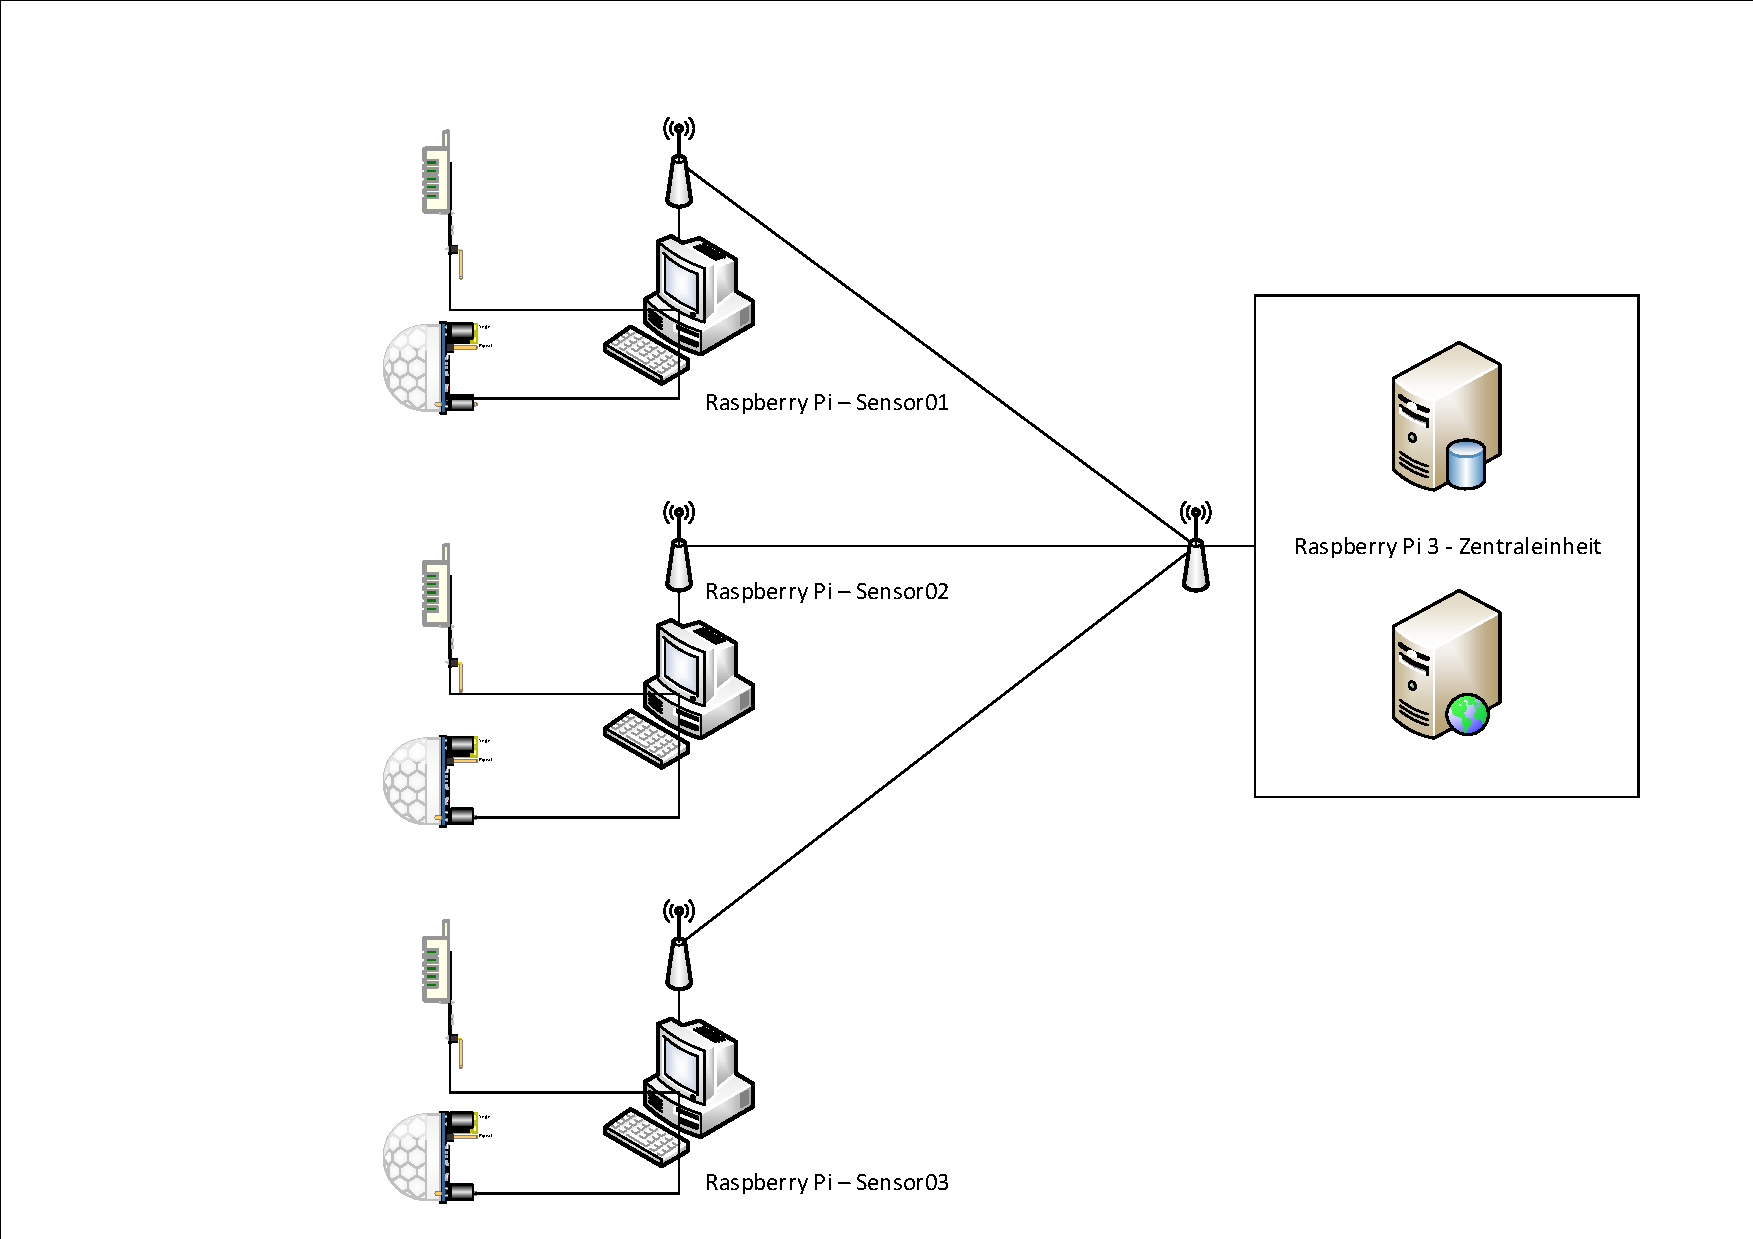
\includegraphics[scale=0.4]{Bilder/Netzplan.pdf}
\caption[Schematische Darstellung der geplanten Umgebung]{Schematische
Darstellung der geplanten Umgebung}
\label{Darstellung_Umgebung}
\end{centering}
\end{figure} 

\subsection{Kommunikation}

\section{Sensorknoten}
Der Raspbarry Pi, an dem die Messdaten der Sensoren gesammelt werden, wird als Sensorknoten bezeichnet. An diesem können bis zu sieben Sensoren, die im Kapitel \nameref{Sensoren_Planung} beschrieben sind, angeschlossen werden. Neben dem Messen muss der Sensorknoten die Messdaten an die Zentraleinheit weiterleiten, welche die Daten auswertet. Bevor der Sensorknoten implementiert werden kann, muss eine Auswahl der Programmiersprache getroffen werden.
\subsection{Python vs. Java}
Für das Projekt ist die richtige Sprache essenziell. Die Sprache muss nicht nur die Daten der Sensoren auslesen, sondern diese auch in Pakete packen und an die Zentraleinheit weitergeben. Die Weitergabe der Datenpackte sollte über eine Schnittstelle erfolgen, die von der ausgewälten Sprache erstellt werden kann. Hierzu wurden zwei Programmiersprachen ausgewählt, \nameref{Java} und \nameref{Python}. Folgende Tabelle zeigt die Funktionaliäten der Sprachen, die für das Projekt notwendig sind:\hfill

\begin{table}[h]
	\centering
	\caption{Python vs. Java}
	\label{my-label}
	\begin{tabular}{lll}
	\textbf{Python} & \textbf{Java} & \textbf{Funktionalität}  \\
	niedrieg & hoch &  Speicherverbrauch\\
	vorhanden & nicht vorhanden & Bibliotheken für die Sensoren \\
	einfach & komplex & Schwierigkeit \\
	hoch & hoch & Geschwindigkeit \\
	vorhanden & vorhanden & Schnittstelle für die Datenübertragung
	\end{tabular}
\end{table}
\noindent Da die Raspberry Pi's für schnelle kleine Hardwarenahe Projekte ausgelegt sind, fiel die Entscheidung auf die Sprache Python, da Java nur bedingt hardwarenah ist und die Speicherkapazität der Raspberry Pi's begrenzt ist. Ein weitere Vorteil von Python, sind die bereits vorhandenen Bibliotheken und die kurze Einarbeitungszeit. Die kürzere Einabreitungs- und Umsetzungszeit, kommt dem engmaschigen Zeitplan zu gute.

\subsection{Auslesen der Sensoren}
%TODO: Priorisierung der Sensoren
%TODO: Allgemeine Messdatenformat
\section{Zentraleinheit}
\subsection{Datenbank}
\subsection{Website}

Auf der Website kann man sich einloggen und einen neuen Benutzer registrieren.
Nach dem Login kommt man auf eine Übersicht auf der alle Sensorknoten in
Tabellenform abgebildet sind mit den aktuell gemessenen Werten. \\
Auf der Statistik-Seite wird ein Verlauf über mehrere Tage zu einem Sensor
abgebildet.\\
Die Webcam-Seite dient dazu, auf die Webcams zuzugreifen, die an den einzelnen Sensorknoten
angeschlossen sind.\\
Das Impressum dient dazu das Projekt kurz zu beschreiben und dieses Dokument
herunterzuladen.\\
Auf der Logout-Seite bekommt man die Meldung, dass man ausgeloggt ist und die
Möglichkeit zurück zur Login-Seite zu kommen.
(\nameref{Darstellung_Website_einfach})


\begin{figure} [htb]
\begin{centering}
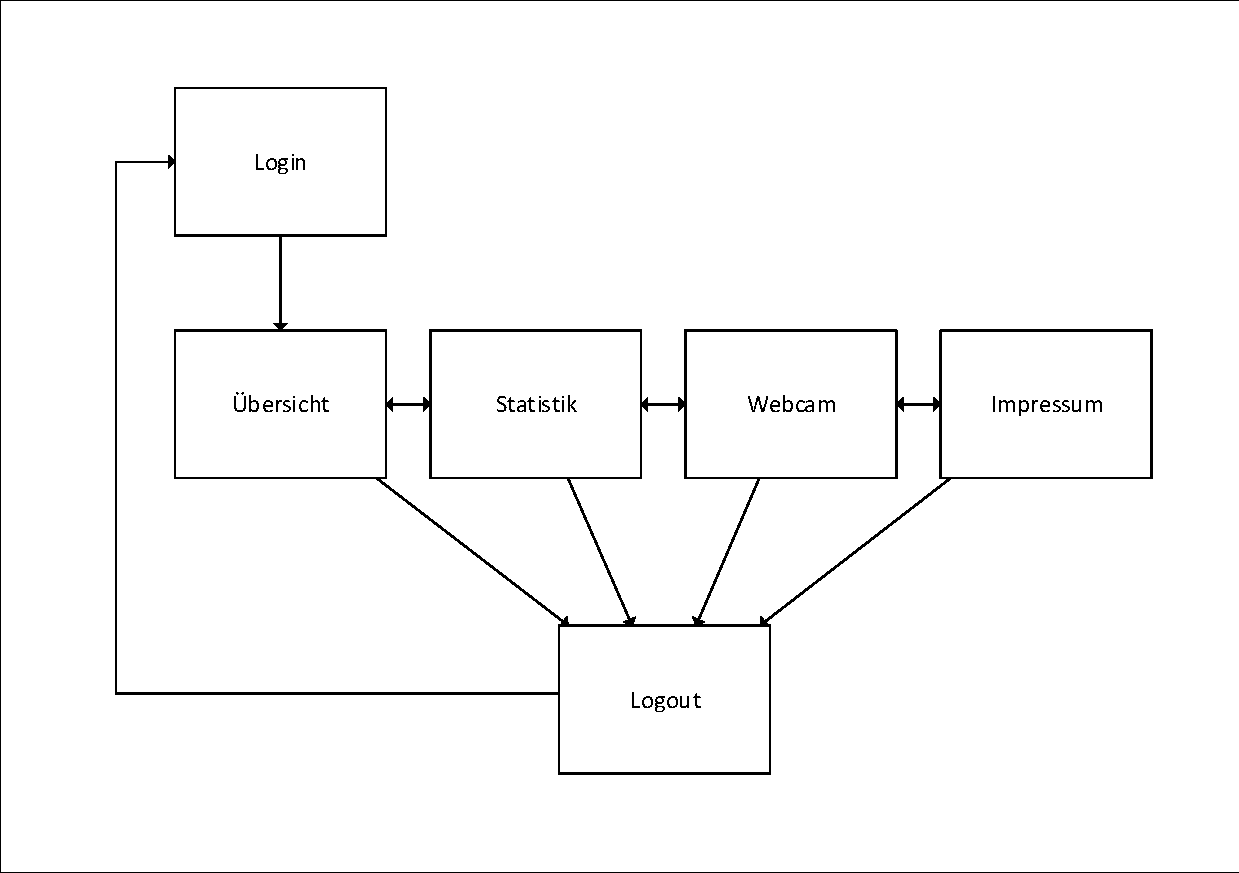
\includegraphics[scale=0.8]{Bilder/struktur_website_einfach.pdf}
\caption[Schematische Darstellung der geplanten Website]{Schematische
Darstellung der geplanten Website}
\label{Darstellung_Website_einfach}
\end{centering}
\end{figure}


\section*{Soll-Zustand}
Die Sensoren werden kontinuierlich abgefragt und senden die gemessenen Werte an
die Datenbank auf der Zentraleinheit. Dort werden die Daten entsprechend dem
meldenden Sensorknoten abgespeichert. Die Website greift auf die Datenbank zu
und lädt die Daten in eine tabellarische Darstellung, die der Benutzer dann
sieht. Durch einen Zeitstempel ist es möglich bei Daten der Temperatursensoren
und der Feuchtigkeitssensoren einen Verlauf darzustellen.

\section*{Datendiagramme}
xfdtrdzhftjgzjfkzjtderdsfrtdrthztjswtqw
